\section{Introduction}
\label{sec:intro}

The need to embed valid strings in one language into valid strings in another
is commonplace throughout programming practice.
Just a few examples include embedding
regular expressions, URIs, SQL queries, or HTML markup
within string constants in general-purpose programming languages;
JavaScript code embedded in HTML via the \verb|<script>| element;
and URIs embedded as query strings within other URIs,
such as in a query to a service like the
\href{https://archive.org/web/}{Wayback Machine}.

An equally-ubiquitous issue arising from this practice
is the need to transform the embedded string --
generally by \emph{escaping} certain characters sensitive
to the ``host'' language and syntactic context --
so that host language processors will not misinterpret embedded text
as host-language text.
For example,
the regular expression \verb|"[^"]*"| matches double-quoted strings,
but when embedded in a C-like language must be written
like \verb|re.match("\"[^\"]*\"")|,
escaping all the embedded instances of double-quote characters,
so that the embedded quotes will not prematurely end the string literal.
Accidentally forgetting necessary escaping
is naturally a common source of syntax errors in manual embedding practice.
\emph{Automated} embedding is also common practice, however,
such as accepting an arbitrary user-entered string on a web form
and embedding it into HTML via a scripting language like PHP.
With automated embedding,
forgetting to escape embedded strings properly
has become an endless source of critical security bugs
such as SQL injection attacks~\cite{clarke12sql}.

In some future evolution
of today's standard programming languages and practices,
could we achieve the ability to embed any valid string
in essentially any language into any other --
\emph{across languages} --
without ever having to escape, or otherwise transform or obfuscate,
the string to be embedded?
Could we make embedding always a simple matter of verbatim ``copy-and-paste''
when done manually,
or a simple matter of concatenation
or filling a ``hole'' in a tempate
when done automatically?
We propose that the answer can and should be \emph{yes} --
though with important challenges, costs, and caveats of course.

We observe that verbatim interlanguage embedding would be achievable if:
(1)
we could standardize across languages
a set of open/close character pairs
we will call \emph{matchers},
such as the parentheses \verb|()|,
square brackets \verb|[]|,
and curly braces \verb|{}|;
and
(2) 
we could impose the universal ``syntactic discipline''
that \emph{matchers must properly match} in nested pairs
throughout any valid string -- without exception --
in any compliant language.
If \emph{plain text} is an unstructured linear sequence of characters
in a character set like ASCII or Unicode,
then we define \emph{matchertext} to be plain text
conforming to the additional syntactic discipline
that ASCII matchers must match.
For example, the strings `\verb|(a{b}c)|' and `\verb|a({'}["])d|'
are valid matchertext,
while the strings
`\verb|(|', `\verb|{a]|', `\verb|[(])|', and `\verb|}{|'
are plain text but are not valid matchertext.

\begin{figure*}[t]
\begin{center}
\begin{small}
\begin{tabular}{ll}
MRI syntax:	& \verb|http[//search.engine/linksto?site=http[//my.site/]&results=50]| \\
URI syntax:	& \verb|http://search.engine/linksto?site=http%3A%2F%2Fmy.site%2F&results=50| \\
\\
MRI syntax:	& \verb|http[//historical.archive/get?site=http[//my.site/]&year=1998]| \\
URI syntax:	& \verb|http://historical.archive/get?site=http%3A%2F%2Fmy.site%2F&year=1998| \\
\end{tabular}
\end{small}
\end{center}
\caption{Example queries containing embedded resource identifiers
	in URI and MRI syntax for comparison.}
\label{fig:search-query}
\end{figure*}

Consider \emph{matchertext resource identifiers} (MRIs),
a matchertext adapation of
uniform resource identifiers (URIs)~\cite{rfc3986} or
internationalized resource identifiers (IRIs)~\cite{rfc3987}.
A URI like \verb|http://my.site/path/|
may always be transformed to or from
equivalent MRI syntax like \verb|http[//my.site/path]|.
An MRI is embeddable verbatim, with no transformation,
into another MRI or another matchertext-aware language.
Figure~\ref{fig:search-query} shows two example search queries
containing embedded resource identifiers,
contrasting ``copy-and-paste'' embeddable MRI syntax
with traditional URI syntax where the sensitive
colon (\verb|:|) and slash (\verb|/|) characters
must be escaped as \verb|%3A| and \verb|%2F%|, respectively.

\begin{figure*}[t]
\begin{center}
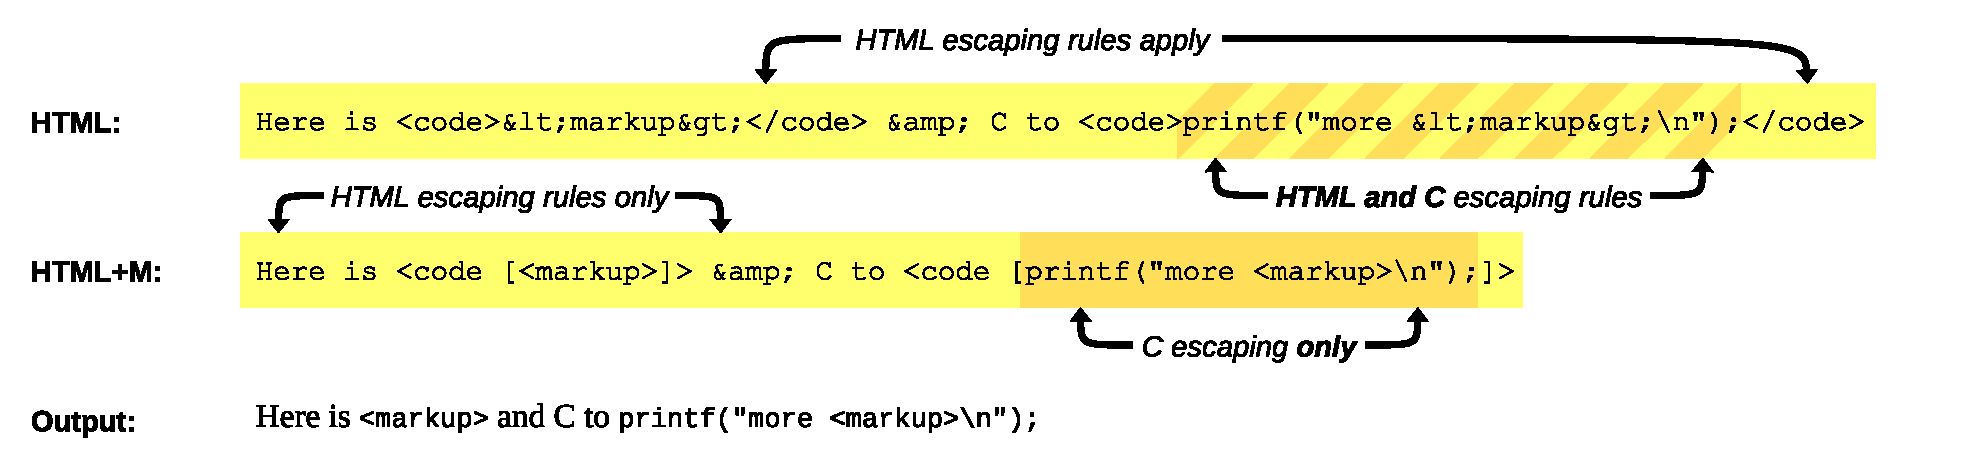
\includegraphics[width=0.95\textwidth]{fig/territorial-integrity.eps}
\end{center}
\caption{Illustration of how different languages' escaping rules
	combine to increase syntactic complexity
	in traditional embedding practice,
	while in matchertext only one language's escaping rules
	are ever active at a given text position.}
\label{fig:territorial-integrity}
\end{figure*}

Adopting the matchertext discipline
does not eliminate the need for character escape sequences:
in fact it can slightly increase the ``escaping obligations''
within a language, as discussed below.
But matchertext enables languages to preserve
the ``territorial integrity'' of their escaping and other syntactic rules,
ensuring that developers need to think about
\emph{only one language's rules at a time}
at any given text position,
even in a string composed from multiple languages.
Thus, matchertext arguably reduces the cognitive load
of writing (or reading) cross-language embedded code.
Figure~\ref{fig:territorial-integrity} illustrates this difference
with a simple example with C code embedded in HTML
including the use of escape codes in both languages.

Existing languages could be adapted incrementally
to support and leverage matchertext.
C-like languages, for example,
might adopt a new escape sequence `\verb|\[|$m$\verb|]|'
to embed an arbitrary matchertext $m$
into a quoted string or character literal.
All characters including quotes and newlines
would be allowed verbatim within $m$,
provided only that matchers match.
Thus,
%\verb|'\[']'| would be equivalent to \verb|'\''|, and
the earlier string-matching regular expression
\verb|"[^"]*"|
could be embedded into a string literal
like \verb|re.match("\["[^"]*"]")|.
We now use an escape sequence
to delimit the entire embedded matchertext,
but we no longer need to add escape sequences
\emph{within} the embedded regular expression.

It is already feasible to write code in existing languages
that is also valid matchertext,
with a bit of care.
Most languages use the matchers in structurally paired forms anyway,
as in expressions like \verb|a*(b+c)|,
lists like \verb|[a,b,c]|,
or maps like \verb|{a:1, b:"hi"}|.
The challenge is mainly in handling the exception cases
where unmatched matchers may commonly appear.

\begin{table*}[t]
\begin{center}
\begin{footnotesize}
\begin{tabular}{ll||ll|ll|ll||ll|ll}
&		& \multicolumn{6}{|l||}{Escapes for C-like languages}
		& \multicolumn{4}{|l}{Escapes for SGML-derived languages} \\
&		& \multicolumn{2}{|l|}{octal escapes}
		& \multicolumn{2}{|l|}{hex escapes}
		& \multicolumn{2}{|l||}{\bf matchers (new)}
		& \multicolumn{2}{|l|}{entity names}
%		& \multicolumn{2}{|l|}{hex}
		& \multicolumn{2}{|l}{\bf matchers (new)}		\\
		&
		& open			& close
		& open			& close
		& open			& close
		& open			& close
		& open			& close		\\
\hline
Parentheses	& \verb|()|
		& \verb|\050|		& \verb|\051|
		& \verb|\x28|		& \verb|\x29|
		& \verb|\o()|		& \verb|\c()|
		& \verb|&lpar;|		& \verb|&rpar;|
%		& \verb|&#x28;|		& \verb|&#x29;|
		& \verb|&o();|		& \verb|&c();|	\\
Square brackets	& \verb|[]|
		& \verb|\133|		& \verb|\135|
		& \verb|\x5B|		& \verb|\x5D|
		& \verb|\o[]|		& \verb|\c[]|
		& \verb|&lbrack;|	& \verb|&rbrack;|
		& \verb|&o[];|		& \verb|&c[];|	\\
		
Curly braces	& \verb|{}|
		& \verb|\173|		& \verb|\175|
		& \verb|\x7B|		& \verb|\x7D|
		& \verb|\o{}|		& \verb|\c{}|
		& \verb|&lbrace;|	& \verb|&rbrace;|
		& \verb|&o{};|		& \verb|&c{};|	\\

\end{tabular}
\end{footnotesize}
\end{center}
\label{tab:unmatched-matchers}
\caption{Potential alternatives in C- and SGML-derived languages
	to escape unmatched matchers in matchertext.}
\end{table*}

One habit we must awkwardly unlearn to write matchertext,
unfortunately,
is using unmatched matchers in quoted strings
to parse or print structured text.
Clauses like \verb|printf("{")| or \verb|case "]"|
are not valid matchertext --
at least not within the string literals.
We must therefore escape these unmatched matchers,
as in \verb|printf("\x7B")| or \verb|case "\x5D"| for example.
Backward-compatible language extensions might ease this pain,
however, 
with new escape sequences that include \emph{both} matchers of a pair
but select only the opener or closer.
The new escape \verb|\o()| represents a literal open parenthesis,
for example,
while \verb|\c[]| represents a close bracket.
Table~\ref{tab:unmatched-matchers} summarizes a few existing and proposed
alternatives for escaping unmatched matchers
in both C-like languages and SGML-derived languages like HTML.

In the rest of this paper, 
we develop more deeply the design and rationale for the matchertext discipline,
then explore how a number of common languages of varying types
might be incrementally adapted to support and leverage
the matchertext discipline effectively.

This work is in an early exploration and experimentation phase,
so the evaluation is currently a placeholder,
serving as a preliminary map for the ways in which
we \emph{would like to} evaluate matchertext
and its use in practical languages.
Some key questions we would like to answer include:
how common (and how painful) is the need for escaping
in the most common cross-language embedding scenarios?
How extensively would large existing repositories of code or data
need to be modified in order to convert them to matchertext?
How does matchertext affect the usability to users or developers
of common constructs in common embedding use-cases,
such as synthesizing or editing HTTP or SQL queries?
How does matchertext affect the frequency of syntax-related bugs --
especially those potentially leading to security vulnerabilities --
in code from typical developers?


\xxx{
Caveats:
- does not eliminate other needs for escaping (just escaping for embedding).
- does not eliminate the need for correct input validation
in automated embedding
(e.g., checking that the input is matchertext
or transforming it into matchertext)),
and thus cannot be expected to eliminate all syntax-related security bugs
of the SQL injection variety.
Mistakes will still happen.
However, we may hope that the consistent and rigorous application
of the matchertext discipline
might significantly increase the robustness of embedding practices
and hence decrease the frequency of such bugs.
XXX to be tested empirically.
}

\xxx{ paper roadmap}


\subsection*{An open research project}

This draft represents a ``work-in-progress'' snapshot
of an experimental open research project.
Anyone with adequate interest, skills, and motivation
is welcome to contribute to this research project,
and potentially become a co-author upon making a substantial contribution.
(Smaller contributions will receive acknowledgments in the final paper.)
To propose a contribution, please use Pull Requests (PRs)
on the project's GitHub repository.
We do not have time and cannot promise to answer all E-mails,
or provide detailed guidance,
before an interested potential contributor has proactively
created and submitted some significant and well-considered contribution.

